%%%%%%%%%%%%%%%%%%%%%%%%%%%
%                         %
%       2016.11.16.       %
%      Stat bead          %
%    Tamás     LATEX      %
%%%%%%%%%%%%%%%%%%%%%%%%%%%

\documentclass[oneside,titlepage,12pt,a4paper]{report}
%\documentclass[12pt]{report}
\usepackage[centertags]{amsmath}
\usepackage{amsfonts}
\usepackage{amsthm}
\usepackage{newlfont}
%\usepackage[ansinew]{inputenc}
\usepackage[magyar]{babel}	
\usepackage[utf8]{inputenc}		
\usepackage{t1enc}				
\usepackage{graphicx}
\usepackage{color}
%\usepackage[colorlinks]{hyperref}
%\usepackage[active,new,noold,marker]{xrcs}
\usepackage{euler}
\usepackage{amssymb,latexsym}
\usepackage{amsmath}
\usepackage{graphics}
\usepackage{algorithm} 
\usepackage{algpseudocode} %ezzel összeakadhat \usepackage{algorithmic} 
%\usepackage{algorithmic} 
\usepackage{rotating}
\usepackage{bigstrut}
\usepackage{subfigure}
\usepackage{appendix}
\usepackage{setspace}
\usepackage{adjustbox}


\newtheorem{theorem}{Theorem}
\newtheorem{corollary}{Corollary}
\newtheorem{lemma}{Lemma}
\newtheorem{proposition}{Proposition}
\newtheorem{definition}{Definition}
\newtheorem{notation}{Notation}

\textwidth=6.truein \textheight=9.truein \hoffset=-.5truein
\voffset=-.8truein

\frenchspacing				
\setlength{\parskip}{\smallskipamount}	
\renewcommand{\appendixtocname}{Függelék}
\renewcommand{\appendixpagename}{Függelék}
\DeclareMathOperator{\grad}{grad}
\DeclareMathOperator{\sgn}{sign}
\DeclareMathOperator{\PRD}{PRD}
\DeclareMathOperator{\CR}{CR}
\newcommand{\conj}[1]{\overline{#1}}

\begin{document}

\begin{center}
	% Title
	\LARGE \textbf{Kognitív rugalmasság vizsgálata különböző változók segítségével}  \\[1.9cm]
\end{center}


\section*{Adatok jellemzése}

A kognitív rugalmasság méréséhez, egy folyamatos szempontváltást igénylő teszt eredményeit használtuk fel. A teszt 0-50 pont között mér, minél magasabb a pontszám, a személy annál könnyebben tudta a különböző feladatokhoz szükséges újabb és újabb nézőpontokat felvenni, annál kevésbé ragadt bele a korábbi stratégiákba, tehát a kognitív rugalmassága annál magasabb. A kognitív rugalmasságot mérő változó értékeit a az adatbázis "rugalmasság" azonosítóval ellátott oszlopában találjuk. 
\par  A figyelmi váltás képességét egy egyszerű választásos reakcióidő segítségével lett mérve, ahol a személyeknek egy jelzőingertől függően az inger színe vagy formája alapján kellett döntést hozni. Az ri változó által megadott adatok a szempontváltást követő első válasz reakcióidejeinek átlaga. A 100 alatti és 1000 feletti reakcióidők még az átlagolás előtt szűrve voltak. Itt a személyenkénti átlagok szerepelnek.
\par Felhasználtuk továbbá a tesztet kitöltött személyek nemét, (az 1 érték jelöli a férfiakat a 2 pedig a nőket), valamint korát. A tesztben kizárólag felnőtt személyek kognitív rugalmasságát mérték. 
\par Az utolsó változó a tesztalany kreativitásához rendel egy mérőszámot. A "kreativitás" azonosító változó értékét egy úgynevezett "szokatlan használat" kreativitás teszten elért pontszám határozza meg. A teszt lényege, az alanynak egy adott tárgy alternatív felhasználási lehetőségeit kell felsorolnia. Értéke a válaszok számától függően 0-tól kezdve (elméletben) bármennyi lehet.

\section*{Alapstatisztikák}

Az adatokat a \texttt{adatok = read.table([az adattábla eléréi útvonala], header=TRUE);} parancs segítségébel tölthettjük be.
A  summary(adatok) parancs futtatása a  következő  alapadatokat  adja.

\begin{figure}[H]
\begin{center}
  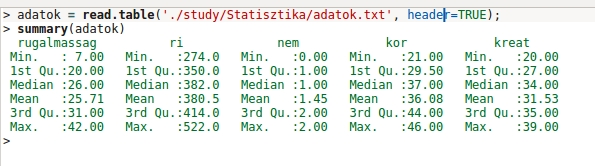
\includegraphics[width=150mm]{./Abrak/summary.jpg}
  \caption{Az summary parancs eredménye}
\end{center}
\end{figure}

Látható, hogy az adatok helyenként javításra szorulnak. Nevezetesen észrevehető, hogy a nemek értékeit tartalmazó oszlop minimuma 0. Tekintettel arra, hogy a nem változó kizárólag az 1 illetve 2 értékeket kaphat, ezért ez az oszlop javításra szorul. Javítás céljából a következő algoritmust alkalmazzuk. Iteráljunk végig a "nemek" oszlop elemein, és amennyiben az elfogadott értékeken kívüli elemet találunk, véletlenszerűen állítsuk az alany nemét férfire illetve nőre. Ezt következő R ciklus segítségével tudjuk elvégezni: 

\begin{figure}[H]
\begin{center}
  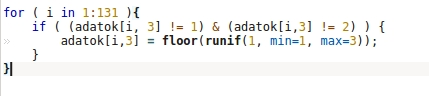
\includegraphics[width=150mm]{./Abrak/cleanDataFunc.jpg}
  \caption{Az adatok javítása}
\end{center}
\end{figure}

Az alábbi ábrából látható, hogy a javítás elvégezte után a summary parancs is elfogadható alapstatisztikákat mutat.

\begin{figure}[H] \label{img::sum2}
\begin{center}
  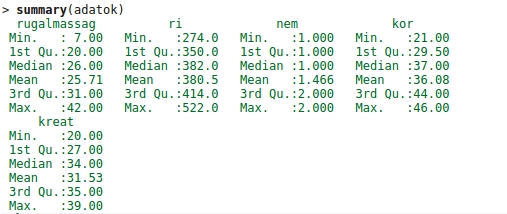
\includegraphics[width=150mm]{./Abrak/cleanDataSum.jpg}
  \caption{A summary parancs eredménye}
\end{center}
\end{figure}


\section*{A rugalmasság és az életkor összefüggése}

Ennek a kísérletnek a célja, hogy megvizsáljuk vajon létezik-e összefüggés a tesztalanyok kora, illetve a kognitív rugalmassági teszten elért pontszámok között. Ezt az összes adaton vizsgáljuk egy másodfokú polinom illesztésével. A függvény-érték párokat illetve a közelítő polinomot az alábbi módon állítjuk elő:

\begin{figure}[H]
\begin{center}
  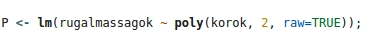
\includegraphics[width=150mm]{./Abrak/policsinal.jpg}
  \caption{A summary parancs eredménye}
\end{center}
\end{figure}

Itt a "rugalmassag" illetve a "korok" vektorok az adatok táblázat megfelelő oszlopait tartalmazzák. Az illesztés elvégzése után, az eredményeket a következő képpen lehet összefoglalni:

\begin{figure}[H]
\begin{center}
  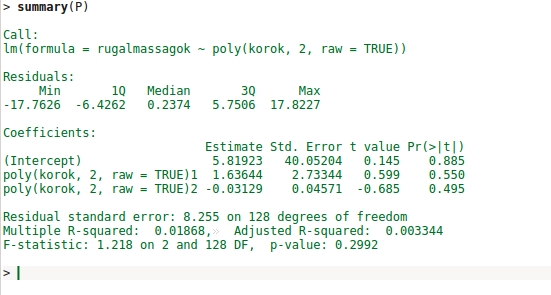
\includegraphics[width=150mm]{./Abrak/polipocs.jpg}
  \caption{A polinom illesztés összefoglalása}
\end{center}
\end{figure}

A nullhipotézisünk ebben az esetben az volt, hogy a polinom együtthatóiként 0 értékeket kapunk. Mivel 95 százalékos konfidencia szintet tekintve mind a  Pr(>|t|)   oszlop   értékei, mind az F-statisztika   p-értéke nagyobb 0,05-nél, ezért elfogadjuk a nullhipotézist. 

\section*{Férfi és női tesztalanyok kognitív rugalmasságának összehasonlítása}

Ebben az kísérletben azt vizsgáltuk, hogy vajon a kognitív rugalmasság pontszámok függetlenek-e a kísérleti alany nemétől. Chi négyzet próba segítségével döntünk a hipotézis helyességéről. Az R nyelv által implementált Chi négyzet próba elvégzéséhez, először létre kell hozni a vizsgált oszlopokat tartalmazó táblázatot. Ezt az alábbi parancs segítségével tehetjük meg.

\begin{figure}[H]
\begin{center}
  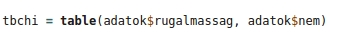
\includegraphics[width=150mm]{./Abrak/chiCreateTable.jpg}
  \caption{Új táblázat létrehozása}
\end{center}
\end{figure}

Ezt követően elvégezhető a beépített Chi négyzet próba. A parancs futtatásakor az R interpreter egy figyelmeztetést ad, mely szerint az elvégzett próba eredménye valószínűleg nem megbízható. 

\begin{figure}[H]
\begin{center}
  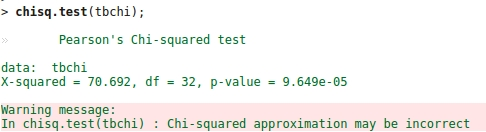
\includegraphics[width=150mm]{./Abrak/chiWarn.jpg}
  \caption{A próba eredménye nem megbízható}
\end{center}
\end{figure}

A megbízhatóbb eredmény érdekében kiegészítjük a fenti parancsot a \texttt{simulate.p.value=T} paraméterrel. A most lefutatott parancs eredménye a következő.

\begin{figure}[H]
\begin{center}
  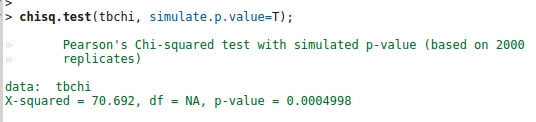
\includegraphics[width=150mm]{./Abrak/chiNoWarn.jpg}
  \caption{A próba eredménye nem megbízható}
\end{center}
\end{figure}

A kapott p-érték (0.0004998) lényegesen alacsonyabb a 0,05-nél ezért elutasítjuk azt a hipotézist, hogy a kognitív rugalmasság a független a nemtől.  


\section*{A kreativitás és a kognitív rugalmasság közötti kapcsolat vizsgálata}

Ebben a kísérletben arra kívánunk választ találni, hogy nevezhetőek-e azonos eloszlásúnak az egyes tesztalanyok által elért kreativitás pontszámok, illetve a kognitív rugalmasság teszten elért pontszámaik. Nullhipotézisként azt tesszük fel, hogy a kreativitás pontszámok és a kognitív rugalmasság teszten elért pontszámok azonos eloszlásúak. A nullhipotézis ellenőrzéséhez Wilcoxon próbát alkalmazunk a következő módon. 


\begin{figure}[H]
\begin{center}
  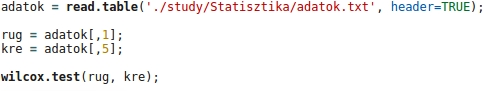
\includegraphics[width=150mm]{./Abrak/wilcoxCommand.jpg}
  \caption{A Wilcoxon próba futtatása}
\end{center}
\end{figure}

Elsőként betöltjük az adatokat. Mivel a vizsgált oszlopok nem szortultak javításra, ezért további teendőnk a próba elvégzése előtt nincs. A sikeres betöltés után, a rugalmasság illetve a kreat oszlopokat értékül adjuk a \texttt{rug} és a \texttt{kre} változóknak. Ezt követően elvégezzük a wilcoxon próbát, amely az alábbi kimenetet produkálja:

\begin{figure}[H]
\begin{center}
  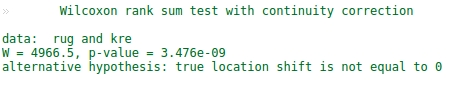
\includegraphics[width=150mm]{./Abrak/wilcoxOutput.jpg}
  \caption{A Wilcoxon próba eredménye}
\end{center}
\end{figure}

A kapott p-érték alapján elutasíthatjuk azt a hipotézist amely szerint a kreativitás pontszámok és a kognitív rugalmasság teszten elért eredmények azonos eloszlásból származnak. Ennek a döntésnek a helyességét szemléltetik az alábbi hisztogrammok is, amelyek rendre a kognitív rugalmasság illetve a kreativitás pontszámok eloszlásait ábrázolják.


\begin{figure}[htb!] \label{fig:eredetiVSsajat}
  \centering
\subfigure[]{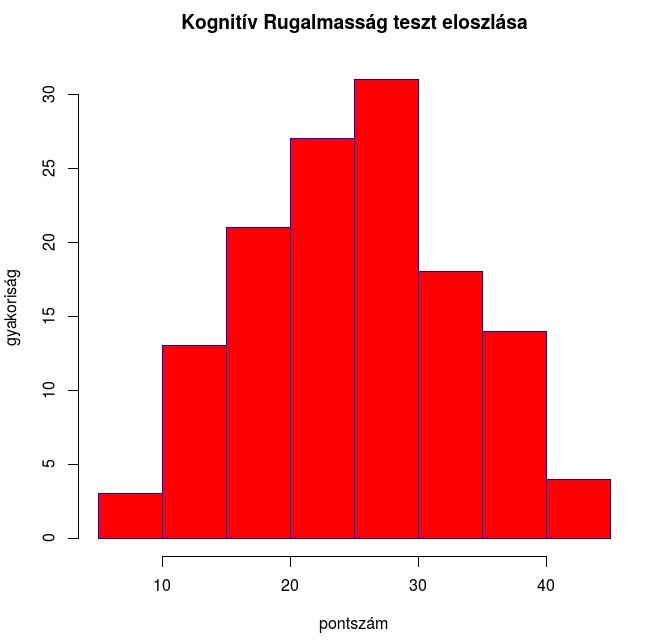
\includegraphics[width=65mm]{./Abrak/histKog.jpg}}
\subfigure[]{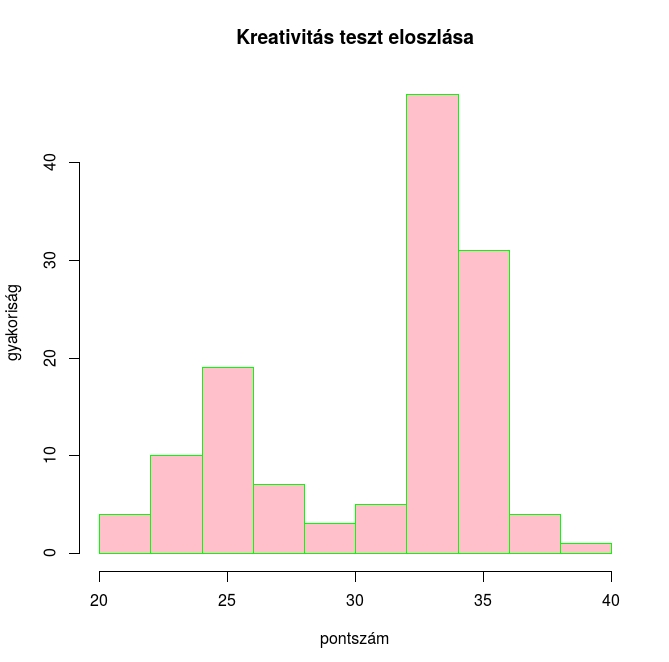
\includegraphics[width=65mm]{./Abrak/histKreat.jpg}}
\end{figure}

\section*{}

\end{document}
